%%%%%%%%%%%%%%%%%%%%%%%%%%%%%%%%%%%%%%%%%
% Beamer Presentation
% LaTeX Template
% Version 1.0 (10/11/12)
%
% This template has been downloaded from:
% http://www.LaTeXTemplates.com
%
% License:
% CC BY-NC-SA 3.0 (http://creativecommons.org/licenses/by-nc-sa/3.0/)
%
%%%%%%%%%%%%%%%%%%%%%%%%%%%%%%%%%%%%%%%%%

%----------------------------------------------------------------------------------------
%	PACKAGES AND THEMES
%----------------------------------------------------------------------------------------

\documentclass{beamer}

\usepackage{helvet}
\renewcommand{\familydefault}{\sfdefault}

\usepackage{inconsolata}
%\usepackage[T1]{fontenc}
%\usepackage{libertine}
\usepackage{listings}
\lstset{language=C++,
  basicstyle=\tiny\ttfamily,
  keywordstyle=\tiny\color{blue}\ttfamily
}

% use Unicode characters - try changing the option if you run into troubles with special characters (e.g. umlauts)
\usepackage[utf8]{inputenc}

% clean citations
\usepackage{cite}

% hyperref makes references clicky. use \url{www.example.com} or \href{www.example.com}{description} to add a clicky url
\usepackage{nameref,hyperref}

\usepackage[export]{adjustbox}


\mode<presentation> {

% The Beamer class comes with a number of default slide themes
% which change the colors and layouts of slides. Below this is a list
% of all the themes, uncomment each in turn to see what they look like.

%\usetheme{default}
%\usetheme{AnnArbor}
\usetheme{Antibes}
%\usetheme{Bergen}
%\usetheme{Berkeley}
%\usetheme{Berlin}
%\usetheme{Boadilla}
%\usetheme{CambridgeUS}
%\usetheme{Copenhagen}
%\usetheme{Darmstadt}
%\usetheme{Dresden}
%\usetheme{Frankfurt}
%\usetheme{Goettingen}
%\usetheme{Hannover}
%\usetheme{Ilmenau}
%\usetheme{JuanLesPins}
%\usetheme{Luebeck}
%\usetheme{Madrid}
%\usetheme{Malmoe}
%\usetheme{Marburg}
%\usetheme{Montpellier}
%\usetheme{PaloAlto}
%\usetheme{Pittsburgh}
%\usetheme{Rochester}
%\usetheme{Singapore}
%\usetheme{Szeged}
%\usetheme{Warsaw}

% As well as themes, the Beamer class has a number of color themes
% for any slide theme. Uncomment each of these in turn to see how it
% changes the colors of your current slide theme.

%\usecolortheme{albatross}
%\usecolortheme{beaver}
%\usecolortheme{beetle}
%\usecolortheme{crane}
%\usecolortheme{dolphin}
%\usecolortheme{dove}
%\usecolortheme{fly}
%\usecolortheme{lily}
%\usecolortheme{orchid}
%\usecolortheme{rose}
%\usecolortheme{seagull}
%\usecolortheme{seahorse}
%\usecolortheme{whale}
%\usecolortheme{wolverine}

%\setbeamertemplate{footline} % To remove the footer line in all slides uncomment this line
%\setbeamertemplate{footline}[page number] % To replace the footer line in all slides with a simple slide count uncomment this line

%\setbeamertemplate{navigation symbols}{} % To remove the navigation symbols from the bottom of all slides uncomment this line

\setbeamertemplate{navigation symbols}{}
}



\usepackage{graphicx} % Allows including images
\usepackage{booktabs} % Allows the use of \toprule, \midrule and \bottomrule in tables
\usepackage{comment}

%----------------------------------------------------------------------------------------
%	TITLE PAGE
%----------------------------------------------------------------------------------------

\title[\textsc{dsgvg}]{Dynamic succinct genome variation graphs} % The short title appears at the bottom of every slide, the full title is only on the title page

\author{Erik Garrison} % Your name
\institute[UCSC] % Your institution as it will appear on the bottom of every slide, may be shorthand to save space
{
University of California, Santa Cruz \\ % Your institution for the title page
\medskip
\textit{erik.garrison@gmail.com} % Your email address
}
\date{\today} % Date, can be changed to a custom date

\begin{document}

\begin{frame}
\titlepage % Print the title page as the first slide
\end{frame}

\begin{frame}
\frametitle{Overview} % Table of contents slide, comment this block out to remove it
\tableofcontents % Throughout your presentation, if you choose to use \section{} and \subsection{} commands, these will automatically be printed on this slide as an overview of your presentation
\end{frame}

%----------------------------------------------------------------------------------------
%	PRESENTATION SLIDES
%----------------------------------------------------------------------------------------

%------------------------------------------------
\section{Variation graphs} % Sections can be created in order to organize your presentation into discrete blocks, all sections and subsections are automatically printed in the table of contents as an overview of the talk
%------------------------------------------------

\subsection{Motivation}

\begin{frame}
  \frametitle{Biological understanding via sequence comparison}
In biology, we are interested in understanding the mutual relations in collections of biosequences (DNA, RNA, and proteins).

\begin{figure}
  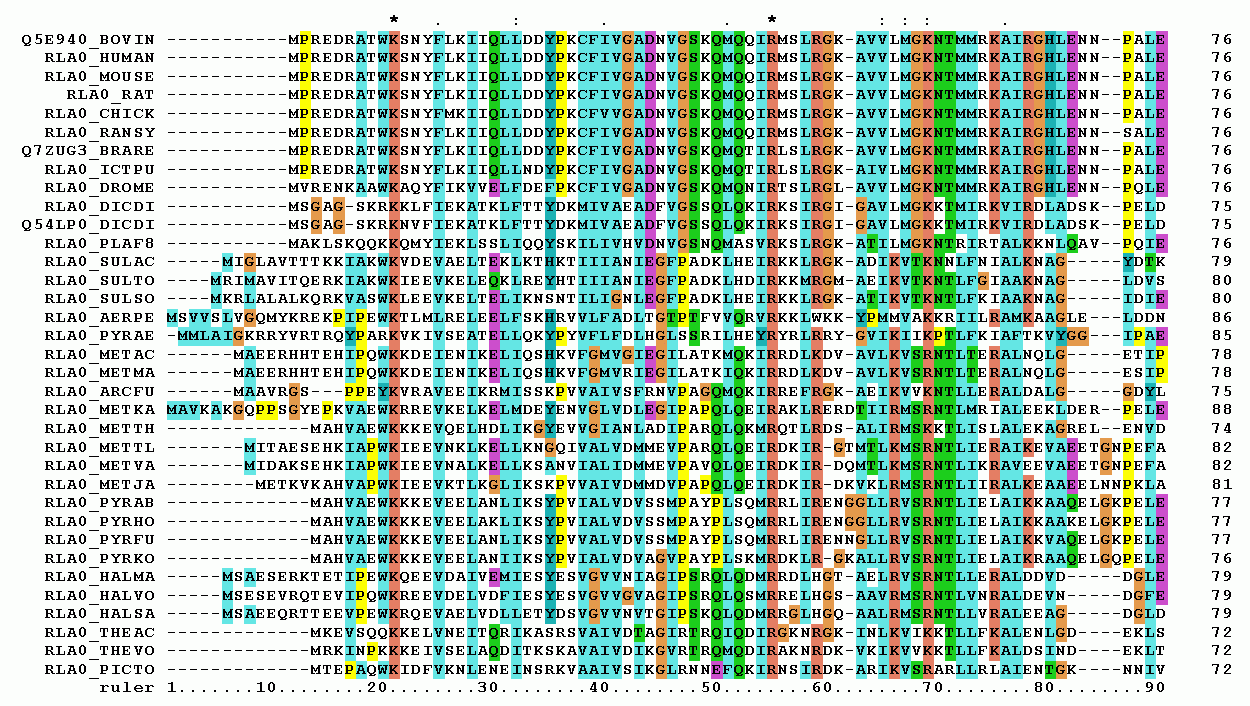
\includegraphics[scale=0.2,center]{RPLP0_90_ClustalW_aln.png}
\end{figure}


\end{frame}

\begin{frame}
    \frametitle{Resequencing}
With large genomes, we have tended to do this via linear reference models.

\begin{figure}
  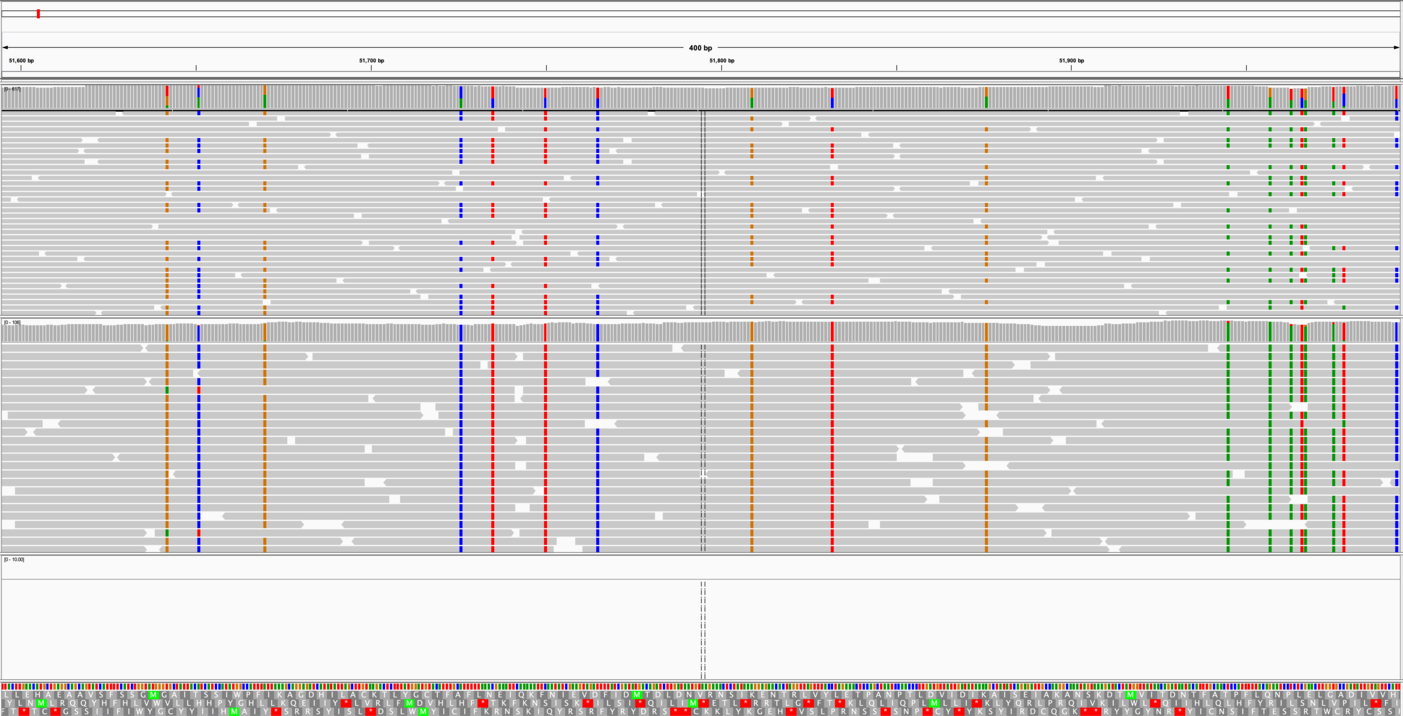
\includegraphics[scale=0.2,center]{TqkY9nw1.png}
\end{figure}
\end{frame}

\begin{frame}
  \frametitle{Reference bias}
  But this can introduce bias.
%  \\~\\
%  The more different an allele is from the reference, the more difficult it is to describe accurately in terms of this reference.

  \begin{figure}
    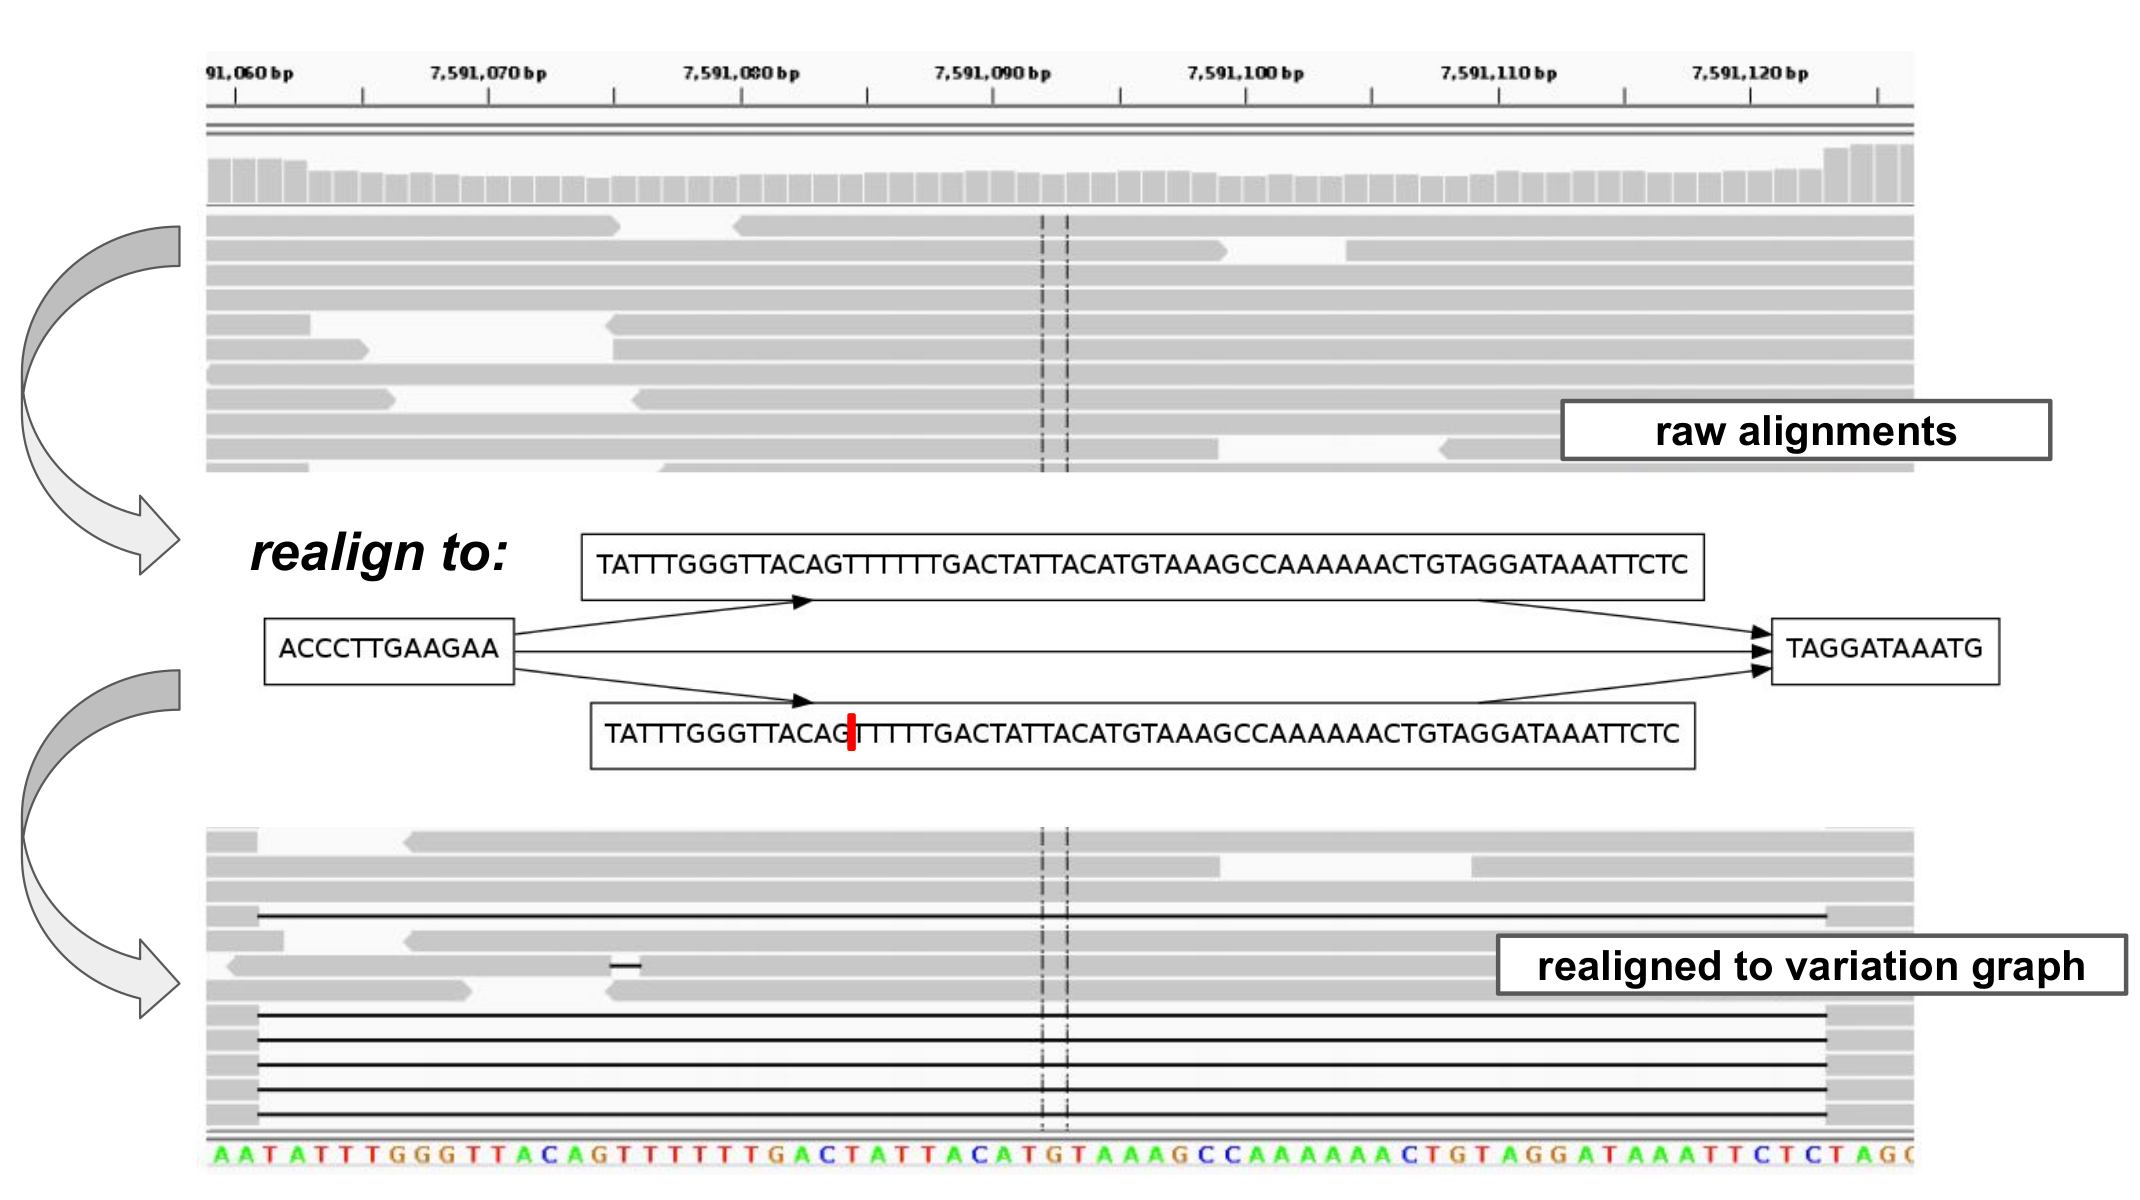
\includegraphics[scale=0.14,center]{igv_graph_realign.png}
    \end{figure}
\end{frame}


\begin{frame}
    \frametitle{Archival ``variant graphs'' project texts into a graph}
%Textual ``variant graphs'' allow the compact description of a set of versions of a text.

    \begin{figure}
      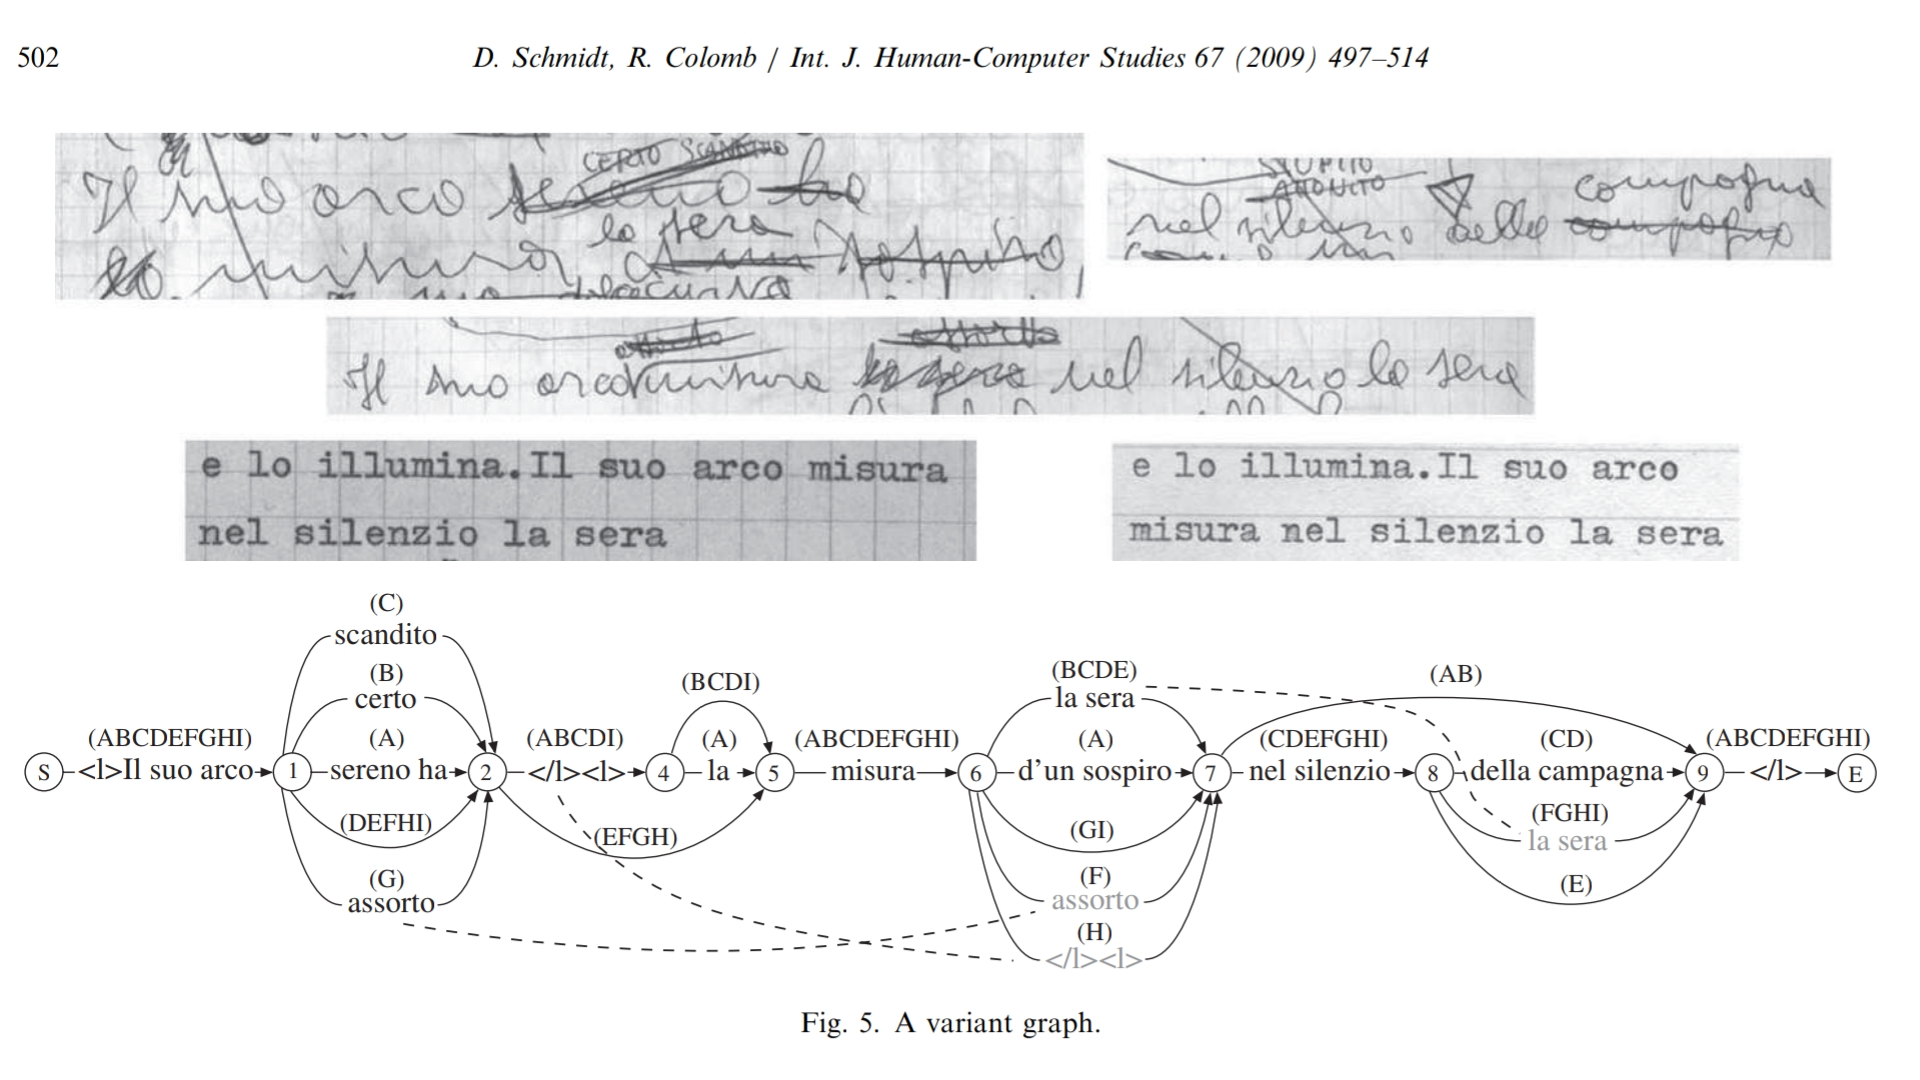
\includegraphics[scale=0.15]{text_variant_graph.jpg}
    \end{figure}
\end{frame}

\begin{frame}
    \frametitle{\emph{Variation graphs} project genomes into a graph}
%Textual ``variant graphs'' allow the compact description of a set of versions of a text.

    \begin{figure}
      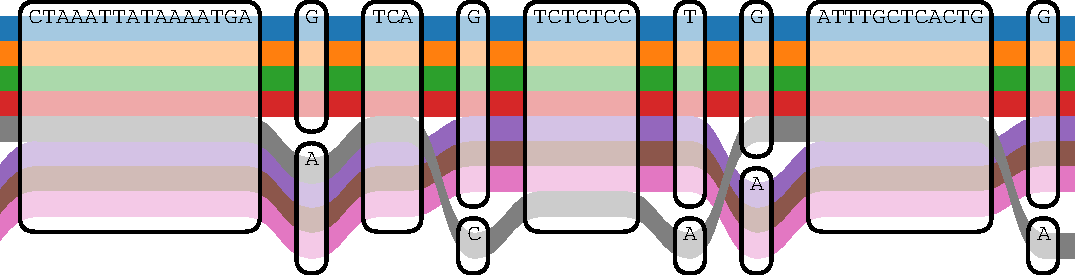
\includegraphics[scale=1.2,center]{vg_tubemap.pdf}
    \end{figure}
\end{frame}

\begin{frame}
  \frametitle{Whole genome alignments}
  \begin{columns}[c] % The "c" option specifies centered vertical alignment while the "t" option is used for top vertical alignment

    \column{.45\textwidth} % Right column and width
    Alignments of whole genomes are equivalently represented as a graph.
    \\~\\
    Here, the variation graph induced by \textsc{seqwish} from the  \textsc{minimap2} alignments of seven \emph{S. cerevisiae} genomes.
    \column{.5\textwidth} % Left column and width

    \begin{figure}
      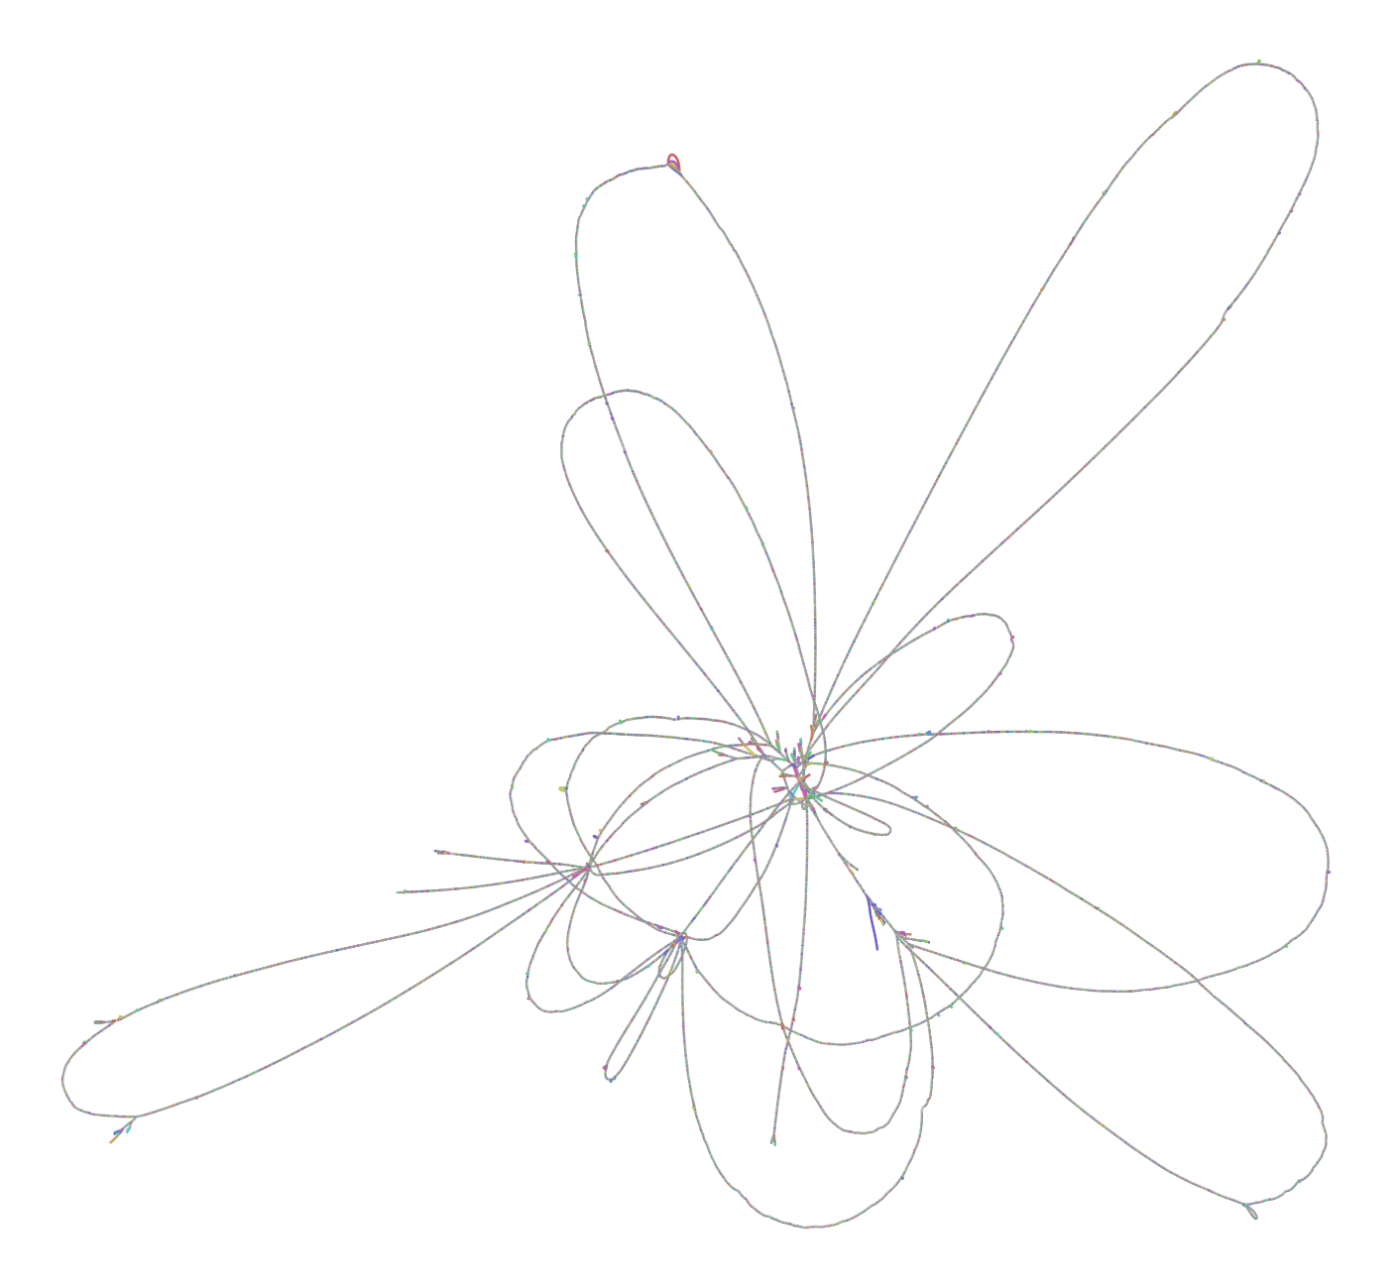
\includegraphics[scale=0.145,center]{seqwish_yeast.png}
    \end{figure}
  \end{columns}
\end{frame}


\subsection{Definitions}

\begin{frame}
  \begin{figure}
    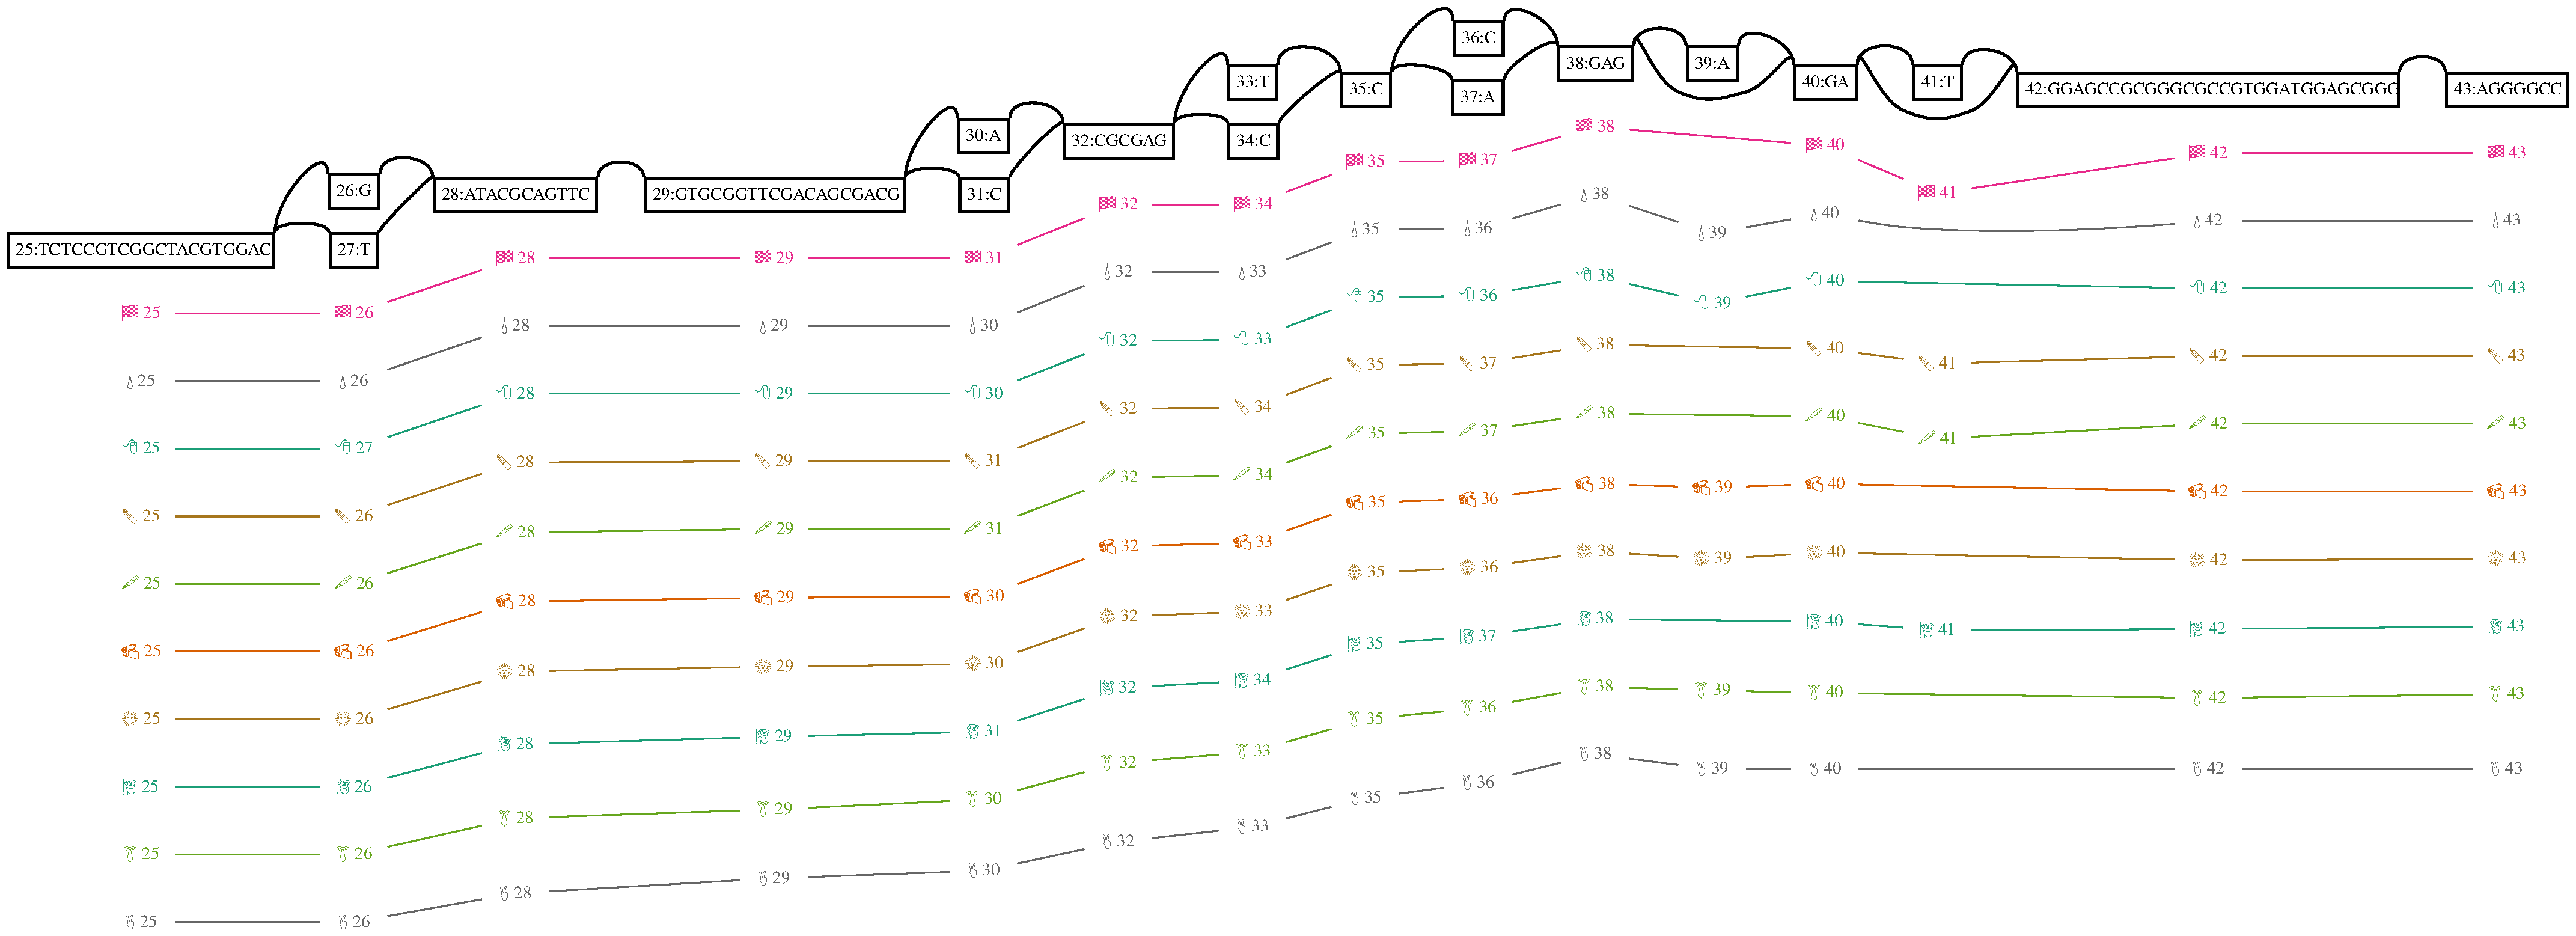
\includegraphics[scale=0.3,center]{H_3136.pdf}
  \end{figure}
\end{frame}

\begin{frame}
  \frametitle{The variation graph model}
  A \emph{variation graph} is a graph with paths: $G = (N, E, P)$.
\\~\\  
  \emph{nodes}: $N = n_1 \ldots n_{|N|}$
  
  \emph{edges}: $E = e_1 \ldots e_{|E|}$

  \emph{paths}: $P = p_1 \ldots p_{|P|}$
  \\~\\
  %Nodes of the graph are labeled with text, and so the nodes and edges can be thought of as a regular language model.
  The graph represents a collection of sequences, with each $p_i$ describing one embedding of a particular sequence within the graph.
  \\~\\
  To model DNA, the graph must be bidirectional and represent both strands of the molecule.
\end{frame}

\begin{frame}
  \frametitle{Nodes are labeled with sequences}
  Each node $n_i$ represents a sequence $seq(n_i)$ that is built from an alphabet $\Sigma = \{ {\tt A, C, G, T, N} \}$.
  \\~\\
  Nodes may be traversed in either the forward or reverse direction, with the sequence being reverse-complemented in the reverse direction.
  \\~\\
  We write $\overline{n_i}$ for the reverse-complement of node $n_i$, so that $seq(n_i) = revcomp(seq(\overline{n_i}))$.
  \\~\\
  Note that $n_i = \overline{\overline{n}}$. For convenience, we refer to both $n_i$ and $\overline{n_i}$ as ``nodes''.
\end{frame}

\begin{frame}
  \frametitle{Edges define allowed paths}
  Edges represent adjacencies between the sequences of the nodes they connect.
  \\~\\
  Thus, the graph implicitly encodes longer sequences as the concatenation of node sequences along walks through the graph.
  \\~\\
  Edges can be identified with the ordered pairs of oriented nodes that they link, so we can write $e_{ij} = (n_i,n_j)$.
  \\~\\
  Edges also can be traversed in either the forward or the reverse direction, with the reverse traversal defined as $\overline{e_{ij}} = (\overline{n_j},\overline{n_i})$.
%  \\~\\
%  VGs can contain ordinary cycles (in which $n_i$ is reachable from $n_i$), reversing cycles (in which $n_i$ is reachable from $\overline{n_i}$), and non-cyclic instances of reversal (in which both $n_i$ and $\overline{n_i}$ are reachable from $n_j$).
  %\\~\\
\end{frame}

%\subsection{Paths are essential}
\begin{frame}
  \frametitle{Paths make the $G$ lossless wrt. sequences}
  If $G = (N, E)$, the graph would do no better than a Markov model at simulating genomes.
  Natural sequences tend to have high long-range mutual information.
%  \\~\\
  \begin{figure}
    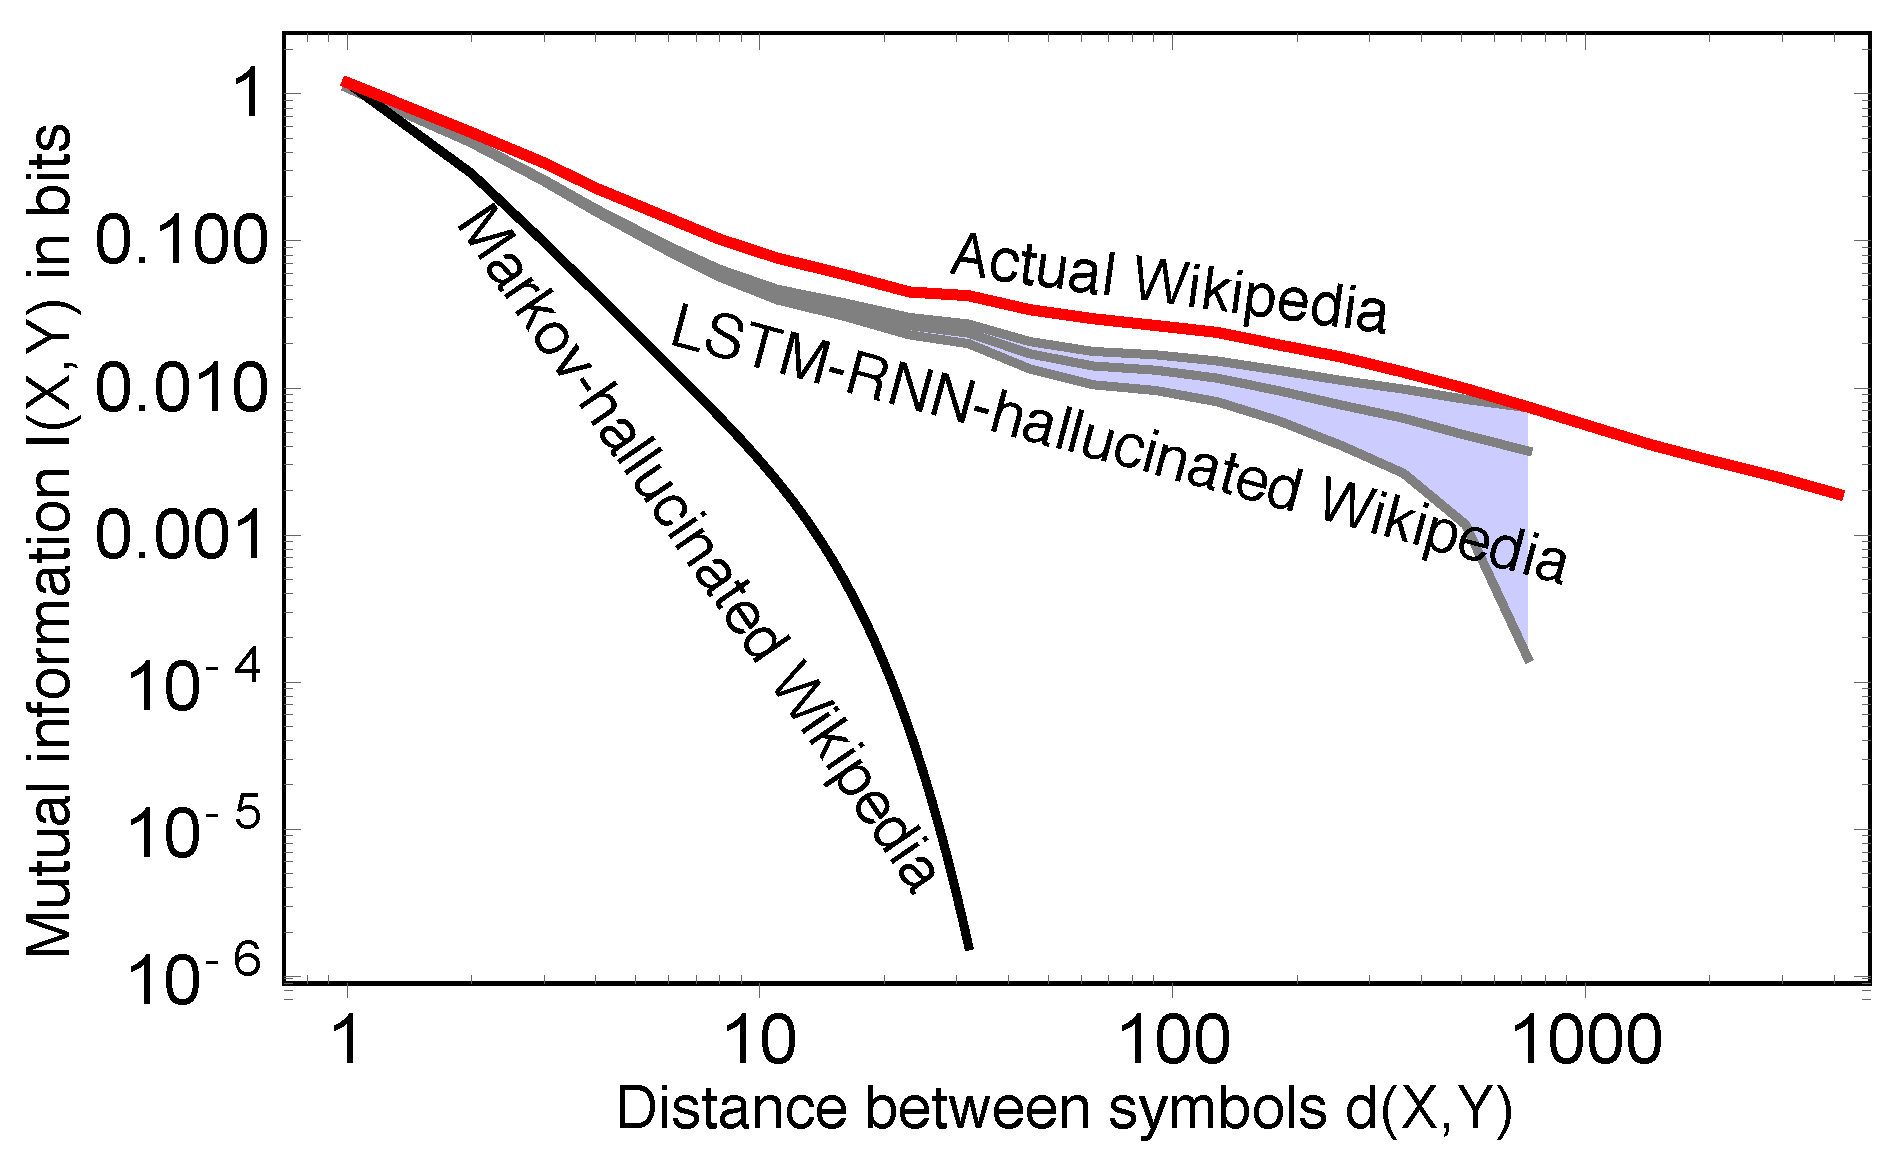
\includegraphics[scale=1,center]{entropy-19-00299-g003.png}
  \end{figure}

  \begin{flushright}
  \tiny{Entropy 2017, 19(7), 299; doi:10.3390/e19070299}
    \end{flushright}
\end{frame}

\section{Representing VGs}

\subsection{Dynamic, uncompressed}

\begin{frame}
  \frametitle{The variation graph toolkit: \textsc{vg}}
    We have implemented variation graph utilities in \textsc{vg}\footnote{\url{https://github.com/vgteam/vg}}.
  \begin{figure}
    
\includegraphics[scale=0.2,center]{vg_logo.png}
  \end{figure}
\end{frame}
  
\begin{frame}[fragile]
  \frametitle{\textsc{vg}'s dynamic graph}
  Represented naïvely, the dynamic graph implemented in \textsc{vg} consumes a lot of memory.
  \\~\\
  Much of it is spent on hash tables and linked lists.
  \\~\\
  For the graph's nodes and edges:
  \begin{lstlisting}
    hash_map<id_t, Node*> node_by_id;
    pair_hash_map<pair<NodeSide, NodeSide>, Edge*> edge_by_sides;
    hash_map<Node*, int> node_index;
    hash_map<Edge*, int> edge_index;
    hash_map<id_t, vector<pair<id_t, bool>>> edges_on_start;
    hash_map<id_t, vector<pair<id_t, bool>>> edges_on_end;
  \end{lstlisting}

  And for the paths $P$.
  
  \begin{lstlisting}
    hash_map<const mapping_t*, pair<list<mapping_t>::iterator, int64_t> > mapping_itr;
    map<string, hash_map<size_t, mapping_t*>> mappings_by_rank;
    hash_map<id_t, map<int64_t, set<mapping_t*>>> node_mapping;
    set<id_t> head_tail_nodes;
  \end{lstlisting}
\end{frame}

\begin{frame}
  \frametitle{Memory woes}
  Loading a variation graph into memory with \textsc{vg}'s default dynamic model can require more than twenty times the uncompressed size in GFA\footnote{\url{https://github.com/GFA-spec/GFA-spec}}.
  \\~\\
  For the human genome and 1000 Genomes Project (1000GP) variation, where the GFA requires 20GB, loading the whole graph is expected to take around 400GB of memory.
\end{frame}

\subsection{Static, succinct}
\begin{frame}[fragile]
  \frametitle{Performant static variation graph}
  To hold large graphs in memory during DNA sequence read alignments, we developed the \textsc{xg} succinct variation graph.
  \\~\\
  The basic idea is to compact the graph into a set of succinct data structures that provide decent cache locality when traversing the graph.
  \\~\\
  This self index is capable of storing the 1000GP graph in 
\end{frame}

\begin{frame}
  \frametitle{\textsc{xg} index of $G = (N, E, P)$}
  The graph is stored in vector $G_\mathbf{iv} = g_1 \ldots g_{|N|}$, with $g_i = ( \eta_i, \Xi_i)$
  \\~\\
  $\eta_i = \left[ id(i), seq_\mathbf{offset}(n_i), |seq(n_i)|, in(n_i), out(n_i) \right]$.
  \\~\\
  $\Xi_i$ is a packed, relativistic recording of the edge context of $n_i$.
  \\~\\
  Bitcompressed vector $S_\mathbf{iv}$ stores the sequence labels of nodes.
  \\~\\
  Paths are recorded in mapping $N_\mathbf{path}$ and a set of per-path vectors that allow for positional and topological queries.
\end{frame}

\begin{frame}
  \frametitle{\textsc{xg} implementation}
  \begin{figure}
    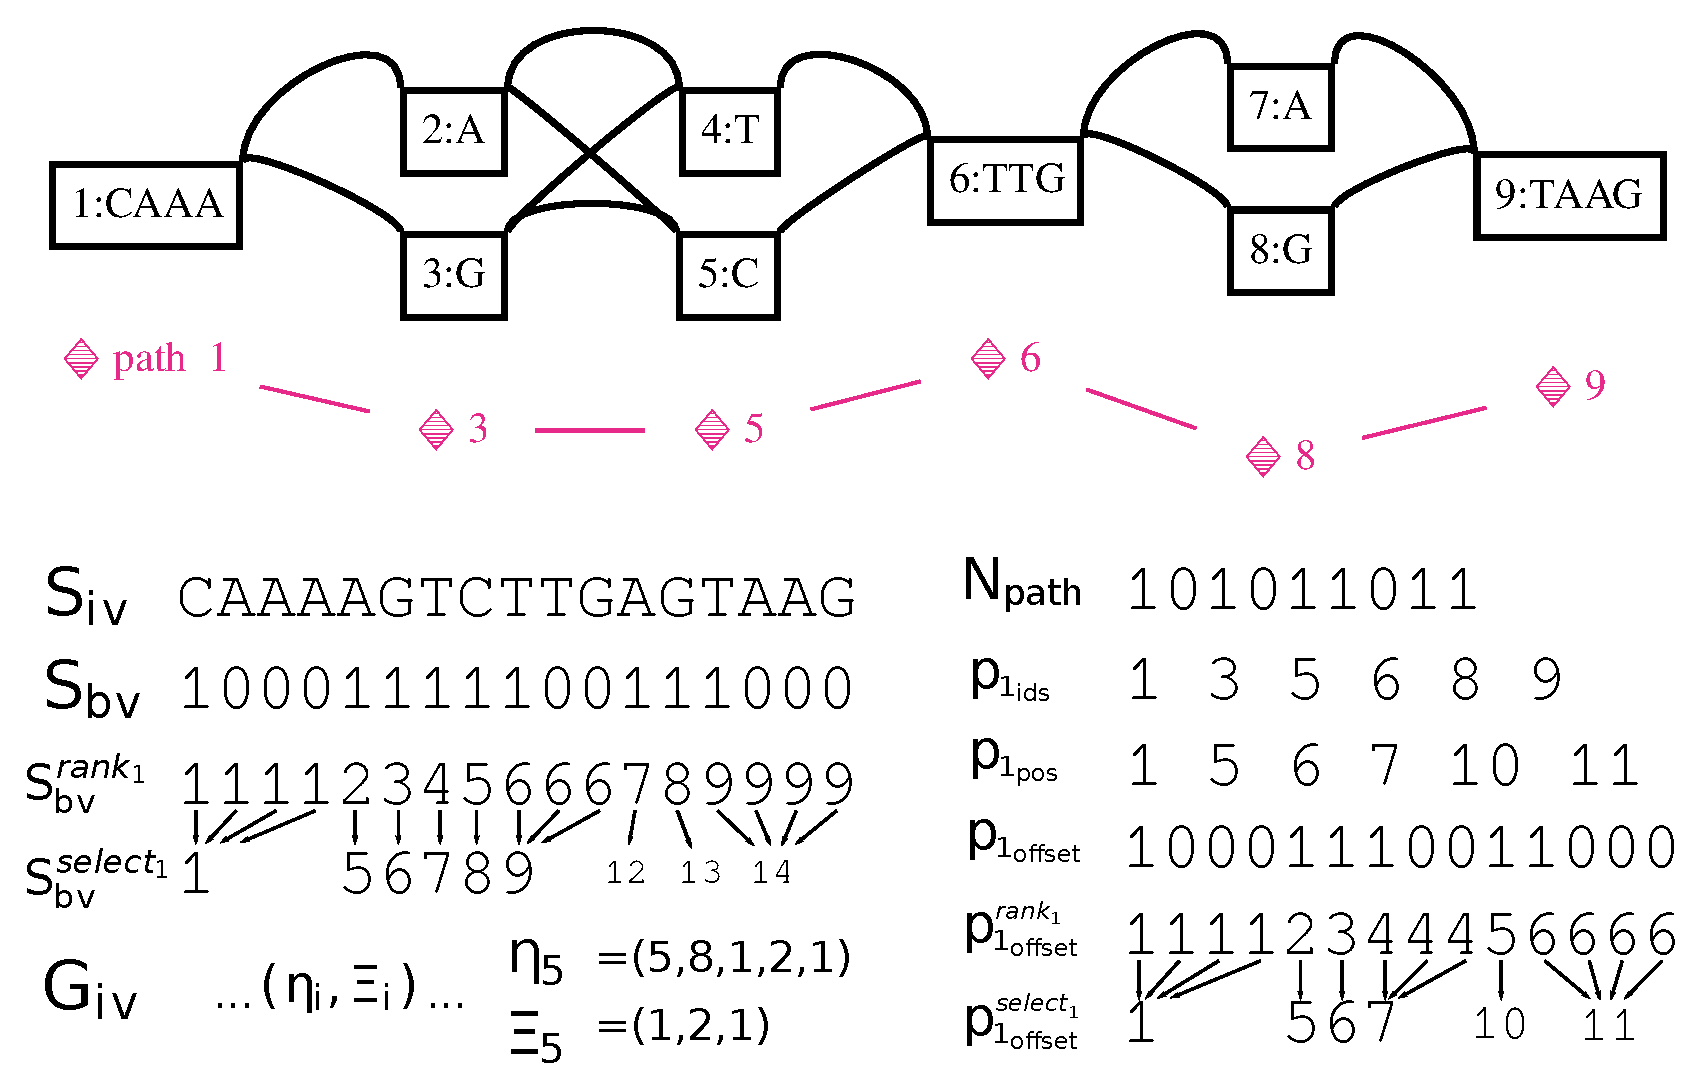
\includegraphics[scale=0.375,center]{xg_index_sketch_nice.pdf}
  \end{figure}
\end{frame}

\begin{frame}
  \frametitle{Succinctly representing haplotypes with the GBWT}
  Sirén's GBWT (and the related gPBWT) use the BWT of haplotypes through the graph to build a compact index of paths.

  \begin{figure}
    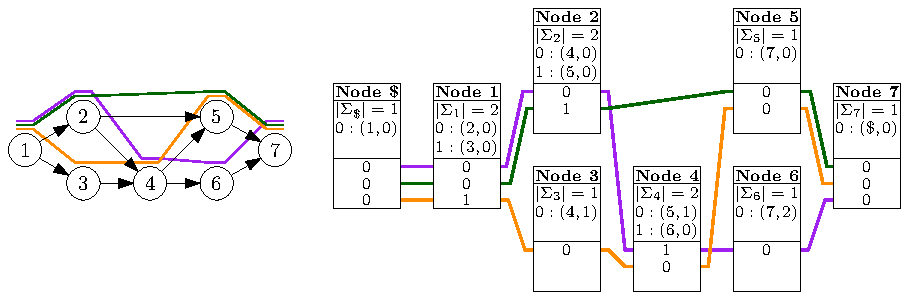
\includegraphics[scale=0.75,center]{gbwt-example.pdf}
  \end{figure}

  The repetitive nature of the paths generated by real genomes makes the GBWT very compressible.
\end{frame}


\section{Dynamic succinct VGs}

%------------------------------------------------

\begin{frame}
\frametitle{Bullet Points}
\begin{itemize}
\item Lorem ipsum dolor sit amet, consectetur adipiscing elit
\item Aliquam blandit faucibus nisi, sit amet dapibus enim tempus eu
\item Nulla commodo, erat quis gravida posuere, elit lacus lobortis est, quis porttitor odio mauris at libero
\item Nam cursus est eget velit posuere pellentesque
\item Vestibulum faucibus velit a augue condimentum quis convallis nulla gravida
\end{itemize}
\end{frame}

%------------------------------------------------

\begin{frame}
\frametitle{Blocks of Highlighted Text}
\begin{block}{Block 1}
Lorem ipsum dolor sit amet, consectetur adipiscing elit. Integer lectus nisl, ultricies in feugiat rutrum, porttitor sit amet augue. Aliquam ut tortor mauris. Sed volutpat ante purus, quis accumsan dolor.
\end{block}

\begin{block}{Block 2}
Pellentesque sed tellus purus. Class aptent taciti sociosqu ad litora torquent per conubia nostra, per inceptos himenaeos. Vestibulum quis magna at risus dictum tempor eu vitae velit.
\end{block}

\begin{block}{Block 3}
Suspendisse tincidunt sagittis gravida. Curabitur condimentum, enim sed venenatis rutrum, ipsum neque consectetur orci, sed blandit justo nisi ac lacus.
\end{block}
\end{frame}

%------------------------------------------------

\begin{frame}
\frametitle{Multiple Columns}
\begin{columns}[c] % The "c" option specifies centered vertical alignment while the "t" option is used for top vertical alignment

\column{.45\textwidth} % Left column and width
\textbf{Heading}
\begin{enumerate}
\item Statement
\item Explanation
\item Example
\end{enumerate}

\column{.5\textwidth} % Right column and width
Lorem ipsum dolor sit amet, consectetur adipiscing elit. Integer lectus nisl, ultricies in feugiat rutrum, porttitor sit amet augue. Aliquam ut tortor mauris. Sed volutpat ante purus, quis accumsan dolor.

\end{columns}
\end{frame}

%------------------------------------------------
\section{Second Section}
%------------------------------------------------

\begin{frame}
\frametitle{Table}
\begin{table}
\begin{tabular}{l l l}
\toprule
\textbf{Treatments} & \textbf{Response 1} & \textbf{Response 2}\\
\midrule
Treatment 1 & 0.0003262 & 0.562 \\
Treatment 2 & 0.0015681 & 0.910 \\
Treatment 3 & 0.0009271 & 0.296 \\
\bottomrule
\end{tabular}
\caption{Table caption}
\end{table}
\end{frame}

%------------------------------------------------

\begin{frame}
\frametitle{Theorem}
\begin{theorem}[Mass--energy equivalence]
$E = mc^2$
\end{theorem}
\end{frame}

%------------------------------------------------

\begin{frame}[fragile] % Need to use the fragile option when verbatim is used in the slide
\frametitle{Verbatim}
\begin{example}[Theorem Slide Code]
\begin{verbatim}
\begin{frame}
\frametitle{Theorem}
\begin{theorem}[Mass--energy equivalence]
$E = mc^2$
\end{theorem}
\end{frame}\end{verbatim}
\end{example}
\end{frame}

%------------------------------------------------

\begin{frame}
\frametitle{Figure}
Uncomment the code on this slide to include your own image from the same directory as the template .TeX file.
%\begin{figure}
%\includegraphics[width=0.8\linewidth]{test}
%\end{figure}
\end{frame}

%------------------------------------------------

\begin{frame}[fragile] % Need to use the fragile option when verbatim is used in the slide
\frametitle{Citation}
An example of the \verb|\cite| command to cite within the presentation:\\~

This statement requires citation \cite{p1}.
\end{frame}

%------------------------------------------------

\begin{frame}
\frametitle{References}
\footnotesize{
\begin{thebibliography}{99} % Beamer does not support BibTeX so references must be inserted manually as below
\bibitem[Smith, 2012]{p1} John Smith (2012)
\newblock Title of the publication
\newblock \emph{Journal Name} 12(3), 45 -- 678.
\end{thebibliography}
}
\end{frame}

%------------------------------------------------

\begin{frame}
\Huge{\centerline{The End}}
\end{frame}

%----------------------------------------------------------------------------------------

\end{document} 
